\documentclass[conference]{IEEEtran}
\IEEEoverridecommandlockouts

\usepackage{cite}
\usepackage{amsmath,amssymb,amsfonts}
\usepackage{graphicx}
\usepackage{textcomp}
\usepackage{xcolor}
\usepackage{booktabs}
\usepackage{hyperref}
\usepackage{url}
\usepackage{array}
\usepackage{multirow}

\hypersetup{
    colorlinks=true,
    linkcolor=blue,
    urlcolor=blue,
    citecolor=blue
}

\def\BibTeX{{\rm B\kern-.05em{\sc i\kern-.025em b}\kern-.08em
    T\kern-.1667em\lower.7ex\hbox{E}\kern-.125emX}}

\begin{document}

\title{Comparative Analysis of Extractive and Abstractive\\
Text Summarization Models on News Articles}

\author{
    \IEEEauthorblockN{[Your Name]}
    \IEEEauthorblockA{
        \textit{Department of [Your Department]}\\
        \textit{[Your University]}\\
        [City, Country]\\
        [your.email@university.edu]
    }
    \and
    \IEEEauthorblockN{[Co-author Name (if any)]}
    \IEEEauthorblockA{
        \textit{Department of [Your Department]}\\
        \textit{[Your University]}\\
        [City, Country]\\
        [coauthor@university.edu]
    }
}

\maketitle

% ─────────────────────────────────────────────────────────────────────
\begin{abstract}
Automatic text summarization is a fundamental task in Natural Language
Processing (NLP) that aims to condense long documents into shorter,
coherent representations while preserving key information. This paper
presents a comparative study of six summarization models --- four
extractive (Lead-3, TextRank, LSA, LexRank) and two abstractive
(T5-small, BART-large-cnn) --- evaluated on the CNN/DailyMail 3.0.0
benchmark dataset. A five-stage preprocessing pipeline was applied to
1,000 test samples, covering HTML cleaning, sentence tokenization, word
tokenization, stop-word removal, and lemmatization. Models were evaluated
using ROUGE-1, ROUGE-2, and ROUGE-L metrics (Precision, Recall, F1).
Results show that BART-large-cnn achieves the highest overall performance
(ROUGE-1 F1: 34.55\%, ROUGE-2 F1: 14.51\%, ROUGE-L F1: 24.69\%), while
the simple Lead-3 baseline remains highly competitive among extractive
methods (ROUGE-1 F1: 29.47\%) due to the inverted-pyramid writing style
of CNN/DailyMail articles. Abstractive models outperform extractive
models by an average of 6.30\% on ROUGE-1 F1. This work provides a
reproducible end-to-end pipeline and a practical comparison to guide
model selection for news summarization tasks.
\end{abstract}

\begin{IEEEkeywords}
Text Summarization, Extractive Summarization, Abstractive Summarization,
ROUGE Evaluation, TextRank, LSA, LexRank, T5, BART, CNN/DailyMail,
Natural Language Processing, Deep Learning
\end{IEEEkeywords}

% ─────────────────────────────────────────────────────────────────────
\section{Introduction}

The exponential growth of digital text --- news articles, research
papers, social media posts, and reports --- has made it increasingly
difficult for users to consume information efficiently. Automatic text
summarization addresses this challenge by generating concise summaries
that retain the most important content from a source document, reducing
reading time while preserving informational value.

Text summarization approaches broadly fall into two categories.
\textbf{Extractive summarization} selects and concatenates the most
relevant sentences directly from the source document. These methods are
computationally efficient and produce grammatically correct output since
they reuse original sentences. \textbf{Abstractive summarization}, on
the other hand, generates new text that may not appear verbatim in the
source, similar to how a human would paraphrase a document. While
abstractive methods can produce more fluent and concise summaries, they
require significantly more computational resources and are prone to
factual hallucinations.

This project implements and compares six models spanning both paradigms
on the CNN/DailyMail dataset \cite{hermann2015} --- one of the most
widely used benchmarks for news summarization. The specific contributions
of this work are:

\begin{enumerate}
    \item A reproducible five-stage preprocessing pipeline for the
          CNN/DailyMail dataset.
    \item From-scratch implementations of four extractive models:
          Lead-3, TextRank, LSA, and LexRank.
    \item Evaluation of two state-of-the-art transformer-based
          abstractive models: T5-small and BART-large-cnn.
    \item A comprehensive comparative analysis using ROUGE-1/2/L
          (Precision, Recall, F1) across all six models.
    \item Per-sample win-rate analysis against the Lead-3 baseline.
\end{enumerate}

The remainder of this paper is organized as follows: Section~\ref{sec:lit}
reviews related work; Section~\ref{sec:method} describes the methodology
including dataset, preprocessing, model implementations, and evaluation;
Section~\ref{sec:conclusion} presents conclusions and future directions.

% ─────────────────────────────────────────────────────────────────────
\section{Literature Review}
\label{sec:lit}

\subsection{Extractive Summarization Methods}

Early work in automatic text summarization dates to Luhn \cite{luhn1958},
who proposed selecting sentences based on word frequency. Edmundson
\cite{edmundson1969} extended this with positional and cue-word features.
These rule-based extractive approaches laid the foundation for graph-based
methods.

\textbf{TextRank} \cite{mihalcea2004} adapted Google's PageRank algorithm
to sentence graphs, where nodes represent sentences and edges represent
cosine similarity between TF-IDF vectors. Sentences with the highest
PageRank scores are selected as the summary. This unsupervised approach
requires no training data and generalizes well across domains.

\textbf{LexRank} \cite{erkan2004} introduced IDF-modified cosine
similarity into the graph construction, giving higher weight to rare but
informative terms. A threshold is applied to remove weak edges, and the
resulting stochastic matrix is used for PageRank scoring. LexRank
consistently outperforms TextRank on news datasets due to its better
handling of term importance.

\textbf{Latent Semantic Analysis (LSA)} for summarization \cite{gong2001}
applies Singular Value Decomposition (SVD) to the TF-IDF sentence-term
matrix to discover latent topics. Sentences are scored by the L2 norm of
their topic vectors, and the top-scoring sentences are selected. LSA
captures semantic relationships beyond surface-level word overlap but is
sensitive to the number of latent components chosen.

The \textbf{Lead-3 baseline} --- selecting the first three sentences of a
news article --- is deceptively strong on CNN/DailyMail due to the
inverted-pyramid journalistic style, where the most newsworthy information
is placed at the beginning. Nallapati et al.\ \cite{nallapati2016}
demonstrated that Lead-3 outperforms many sophisticated extractive models
on this dataset.

\subsection{Abstractive Summarization Methods}

The shift to neural abstractive summarization began with
sequence-to-sequence models \cite{sutskever2014,bahdanau2015}. Rush et
al.\ \cite{rush2015} applied attention-based encoder-decoder models to
headline generation. See et al.\ \cite{see2017} introduced the
Pointer-Generator Network with a coverage mechanism to reduce repetition
and enable copying from the source.

\textbf{T5 (Text-to-Text Transfer Transformer)} \cite{raffel2020}
reframes all NLP tasks as text-to-text problems. The model is pre-trained
on the Colossal Clean Crawled Corpus (C4) with a masked span prediction
objective. For summarization, the input is prefixed with
\texttt{summarize:} and the model generates the summary autoregressively.
T5-small ($\sim$60M parameters, $\sim$240\,MB) is the smallest variant,
making it suitable for resource-constrained environments.

\textbf{BART (Bidirectional and Auto-Regressive Transformers)}
\cite{lewis2020} combines a bidirectional encoder (like BERT) with an
autoregressive decoder (like GPT). It is pre-trained by corrupting text
with various noise functions and learning to reconstruct the original. The
\texttt{facebook/bart-large-cnn} checkpoint ($\sim$400M parameters,
$\sim$1.6\,GB) is fine-tuned directly on the CNN/DailyMail dataset,
giving it a significant advantage on this benchmark. BART has become the
de facto standard for news summarization and consistently achieves
state-of-the-art ROUGE scores.

Recent advances include PEGASUS \cite{zhang2020}, which uses gap-sentence
generation as a pre-training objective specifically designed for
summarization. However, BART-large-cnn remains a strong and widely
reproduced baseline for single-document news summarization.

% ─────────────────────────────────────────────────────────────────────
\section{Methodology}
\label{sec:method}

\subsection{Abbreviations and Acronyms}

Table~\ref{tab:abbrev} lists the abbreviations used throughout this paper.

\begin{table}[h]
\caption{Abbreviations and Acronyms}
\label{tab:abbrev}
\centering
\begin{tabular}{ll}
\toprule
\textbf{Abbreviation} & \textbf{Full Form} \\
\midrule
NLP    & Natural Language Processing \\
ROUGE  & Recall-Oriented Understudy for Gisting Evaluation \\
TF-IDF & Term Frequency--Inverse Document Frequency \\
SVD    & Singular Value Decomposition \\
LSA    & Latent Semantic Analysis \\
T5     & Text-to-Text Transfer Transformer \\
BART   & Bidirectional and Auto-Regressive Transformers \\
CNN/DM & CNN/DailyMail Dataset \\
F1     & F1-Score (harmonic mean of Precision and Recall) \\
GPU    & Graphics Processing Unit \\
CPU    & Central Processing Unit \\
\bottomrule
\end{tabular}
\end{table}

\noindent\textbf{Dataset.}
The CNN/DailyMail 3.0.0 dataset \cite{hermann2015,nallapati2016} contains
approximately 300,000 English news articles paired with human-written
bullet-point summaries (``highlights''). It is hosted on HuggingFace
(\texttt{ccdv/cnn\_dailymail}). For this study, 1,000 samples from the
test split were used for extractive evaluation and 200 samples for
abstractive evaluation (due to CPU inference time constraints).

Table~\ref{tab:datastats} summarises the dataset statistics computed over
the 1,000 test samples used in this study.

\begin{table}[h]
\caption{Dataset Statistics (1,000 Test Samples)}
\label{tab:datastats}
\centering
\begin{tabular}{lcccc}
\toprule
\textbf{Statistic} & \textbf{Sents} & \textbf{Words (Orig.)} &
\textbf{Words (Proc.)} & \textbf{Words (Ref.)} \\
\midrule
Mean & 33.4  & 626.3  & 339.4  & 34.6 \\
Std  & 19.8  & 352.0  & 188.5  & 9.7  \\
Min  & 4     & 73     & 43     & 9    \\
Max  & 112   & 1,750  & 1,326  & 71   \\
\bottomrule
\end{tabular}
\end{table}

\noindent\textbf{Preprocessing Pipeline.}
A five-stage pipeline was applied to all articles:
\begin{enumerate}
    \item \textbf{Cleaning} --- HTML tags, CNN byline prefixes (e.g.,
          \texttt{(CNN) -{}-}), and special characters were removed using
          regular expressions. Extra whitespace was normalized.
    \item \textbf{Sentence Tokenization} --- \texttt{nltk.sent\_tokenize}
          was applied to the cleaned text to split articles into individual
          sentences.
    \item \textbf{Word Tokenization} --- \texttt{nltk.word\_tokenize} was
          applied per sentence to produce word-level tokens.
    \item \textbf{Stop-word Removal} --- NLTK's English stop-word list was
          used to filter non-content words.
    \item \textbf{Normalization} --- All tokens were lowercased and
          lemmatized using \texttt{WordNetLemmatizer}. Non-alphabetic
          tokens were discarded.
\end{enumerate}

Preprocessing reduced the average word count from 626.3 to 339.4 words
per article (a 45.8\% reduction), retaining only content-bearing terms
for model input.

\subsection{Model Implementations}

\noindent\textbf{Lead-3 (Baseline):}
Returns the first three sentences of the cleaned article. No training or
computation is required. Exploits the inverted-pyramid structure of news
writing.

\noindent\textbf{TextRank:}
Sentences are vectorized using TF-IDF. A cosine similarity matrix is
computed between all sentence pairs, and self-similarity is set to zero.
A weighted undirected graph is constructed using NetworkX, and PageRank
(\texttt{max\_iter=300}, \texttt{tol=1e-5}) is applied to score
sentences. The top-3 sentences by score are returned in their original
order.

\noindent\textbf{LSA:}
Sentences are vectorized using TF-IDF (\texttt{max\_features=5,000}).
TruncatedSVD is applied with $k = \min(5,\, n_{\text{sents}}-1,\,
n_{\text{terms}}-1)$ latent components. Each sentence is scored by the
L2 norm of its topic vector. The top-3 sentences are returned in original
order.

\noindent\textbf{LexRank:}
IDF values are computed over all sentences in the article. An
IDF-weighted cosine similarity matrix is built between all sentence pairs.
Similarities below a threshold of 0.1 are set to zero. The matrix is
row-normalized to form a stochastic matrix. PageRank is applied to score
sentences, and the top-3 are returned in original order.

\noindent\textbf{T5-small:}
The HuggingFace \texttt{transformers} pipeline is used with model
\texttt{t5-small}. Each article is truncated to 600 words and prefixed
with \texttt{summarize:}. Beam search (\texttt{num\_beams=4}) is used
with \texttt{max\_length=150}, \texttt{min\_length=40}. Inference runs
in batches of 4 on CPU.

\noindent\textbf{BART-large-cnn:}
The HuggingFace \texttt{transformers} pipeline is used with model
\texttt{facebook/bart-large-cnn}. Articles are truncated to 600 words.
Beam search (\texttt{num\_beams=4}) is used with \texttt{max\_length=142},
\texttt{min\_length=56}, \texttt{length\_penalty=2.0}. Inference runs in
batches of 4 on CPU.

\noindent\textbf{Evaluation Metric.}
ROUGE \cite{lin2004} is the standard metric for summarization evaluation.
It measures $n$-gram overlap between the generated summary and the human
reference:
\begin{itemize}
    \item \textbf{ROUGE-1}: Unigram overlap.
    \item \textbf{ROUGE-2}: Bigram overlap.
    \item \textbf{ROUGE-L}: Longest Common Subsequence (LCS).
\end{itemize}
Each metric reports Precision, Recall, and F1. The \texttt{rouge-score}
library with \texttt{use\_stemmer=True} was used for all evaluations.

\subsection{Results: Figures and Tables}

Table~\ref{tab:rouge} presents the full ROUGE score comparison across all
six models. BART-large-cnn achieves the highest F1 scores on all three
ROUGE metrics. Among extractive models, Lead-3 performs best, followed
closely by LexRank and TextRank. LSA is the weakest model overall.

\begin{table}[h]
\caption{ROUGE Score Comparison --- All 6 Models}
\label{tab:rouge}
\centering
\setlength{\tabcolsep}{4pt}
\begin{tabular}{llccccc}
\toprule
\textbf{Model} & \textbf{Type} & \textbf{R1-P} & \textbf{R1-R} &
\textbf{R1-F1} & \textbf{R2-F1} & \textbf{RL-F1} \\
\midrule
Lead-3    & Ext. & 22.72 & 46.84 & 29.47 & 11.21 & 19.96 \\
TextRank  & Ext. & 20.74 & 44.57 & 27.28 &  9.24 & 18.42 \\
LSA       & Ext. & 19.54 & 30.45 & 22.50 &  5.91 & 15.28 \\
LexRank   & Ext. & 21.49 & 42.29 & 27.42 &  8.80 & 18.28 \\
T5-small  & Abs. & 29.31 & 35.35 & 31.38 & 11.90 & 22.53 \\
\textbf{BART} & \textbf{Abs.} & \textbf{29.06} & \textbf{44.90} &
\textbf{34.55} & \textbf{14.51} & \textbf{24.69} \\
\bottomrule
\multicolumn{7}{l}{\small All values in \%. Ext.=Extractive (n=1000),
Abs.=Abstractive (n=200).}
\end{tabular}
\end{table}

Table~\ref{tab:winrate} shows the per-sample win-rate of each model
against the Lead-3 baseline on ROUGE-1 F1 (evaluated on the 200-sample
overlap). BART wins 69.0\% of comparisons, while LSA wins only 33.5\%,
confirming Lead-3 as a strong extractive baseline.

\begin{table}[h]
\caption{Win-Rate vs.\ Lead-3 Baseline (ROUGE-1 F1, $n=200$)}
\label{tab:winrate}
\centering
\begin{tabular}{lcccc}
\toprule
\textbf{Model} & \textbf{Wins} & \textbf{Losses} & \textbf{Ties} &
\textbf{Win\%} \\
\midrule
TextRank  &  91 & 105 & 4 & 45.5 \\
LSA       &  67 & 133 & 0 & 33.5 \\
LexRank   &  89 & 109 & 2 & 44.5 \\
T5-small  & 113 &  87 & 0 & 56.5 \\
\textbf{BART} & \textbf{138} & \textbf{61} & \textbf{1} & \textbf{69.0} \\
\bottomrule
\end{tabular}
\end{table}

Fig.~\ref{fig:barchart} shows the grouped bar chart of ROUGE-1, ROUGE-2,
and ROUGE-L F1 scores for all six models. BART leads across all metrics.
Fig.~\ref{fig:boxplot} shows the per-sample ROUGE-1 F1 distributions as
box plots. BART exhibits the highest median with relatively low variance,
while LSA shows the lowest median. Fig.~\ref{fig:preproc} shows the word
count distributions at each preprocessing stage.

\begin{figure}[h]
    \centering
    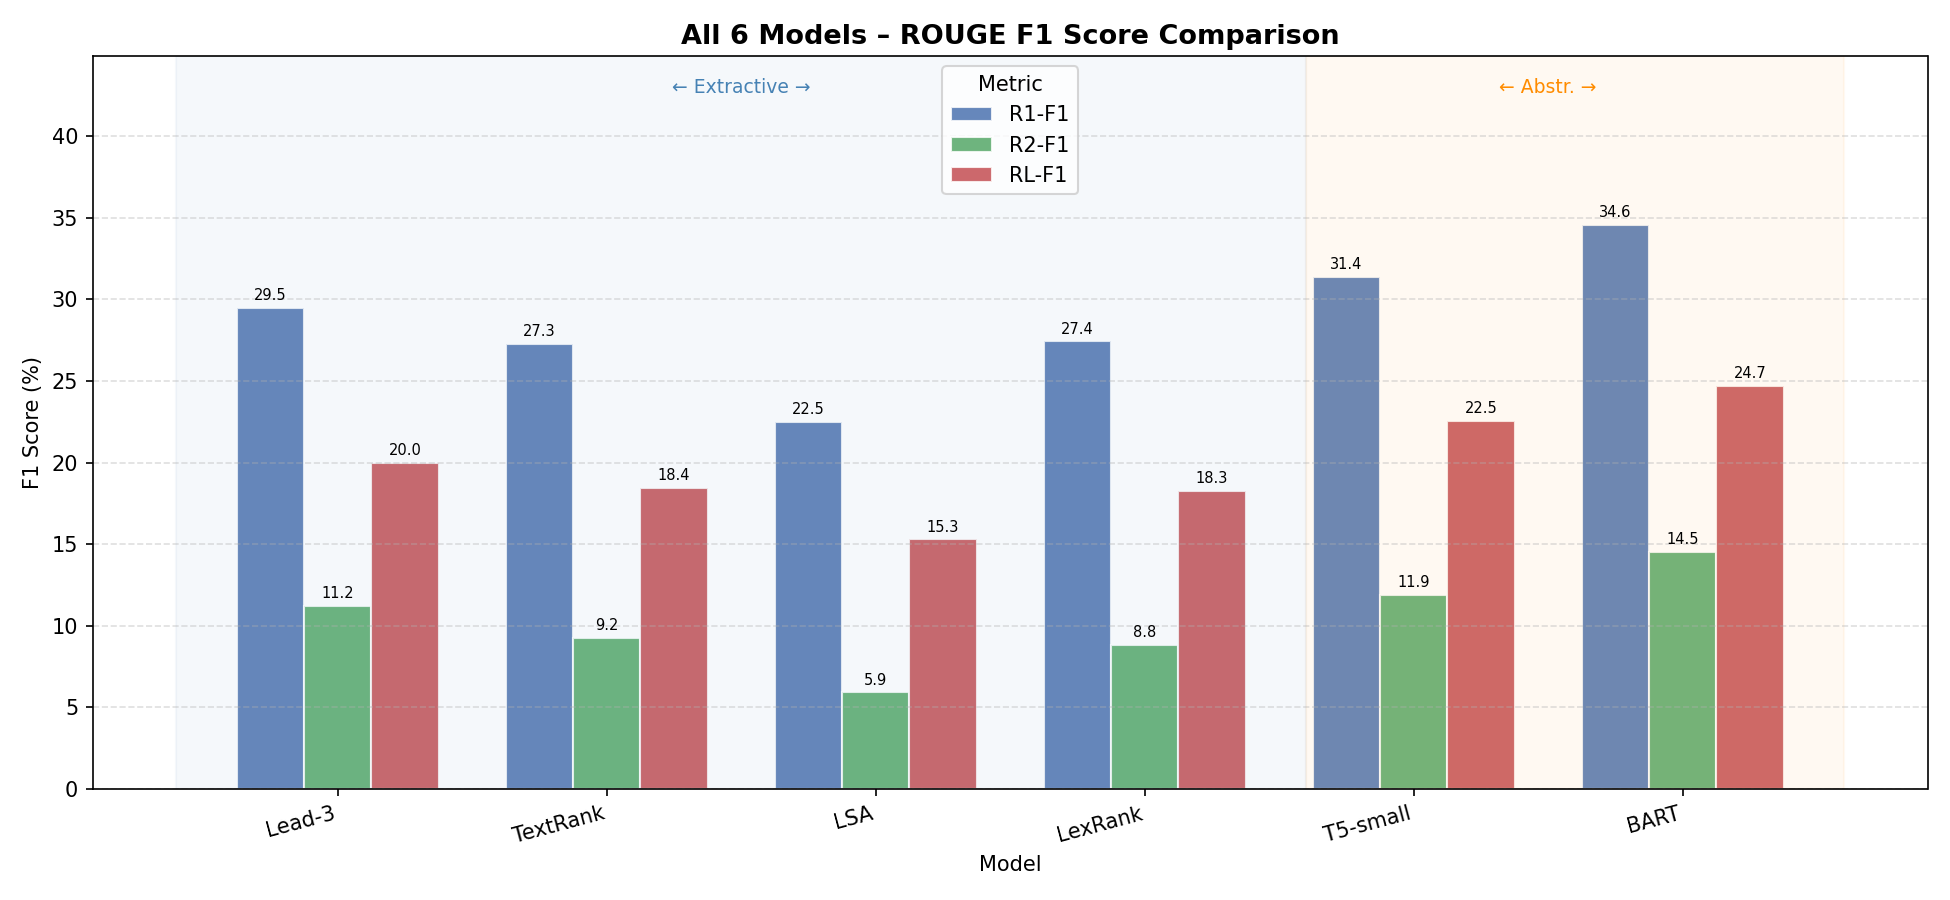
\includegraphics[width=\columnwidth]{outputs/rouge_comparison.png}
    \caption{ROUGE-1, ROUGE-2, and ROUGE-L F1 scores for all six models.
             BART achieves the highest scores across all metrics.}
    \label{fig:barchart}
\end{figure}

\begin{figure}[h]
    \centering
    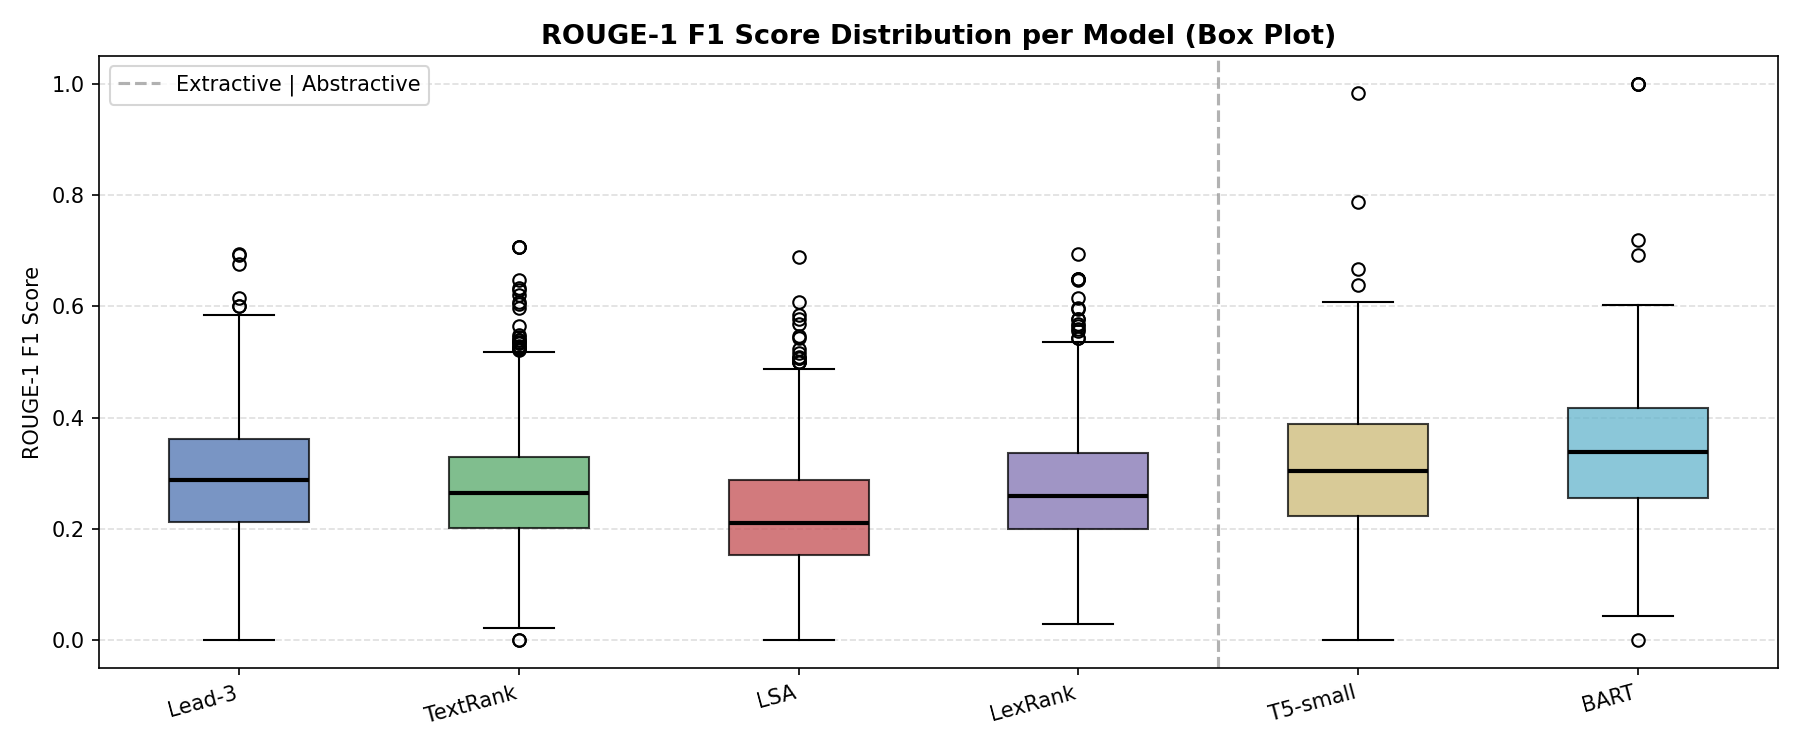
\includegraphics[width=\columnwidth]{outputs/rouge_boxplot.png}
    \caption{Per-sample ROUGE-1 F1 score distributions (box plots).
             The dashed vertical line separates extractive (left) from
             abstractive (right) models.}
    \label{fig:boxplot}
\end{figure}

\begin{figure}[h]
    \centering
    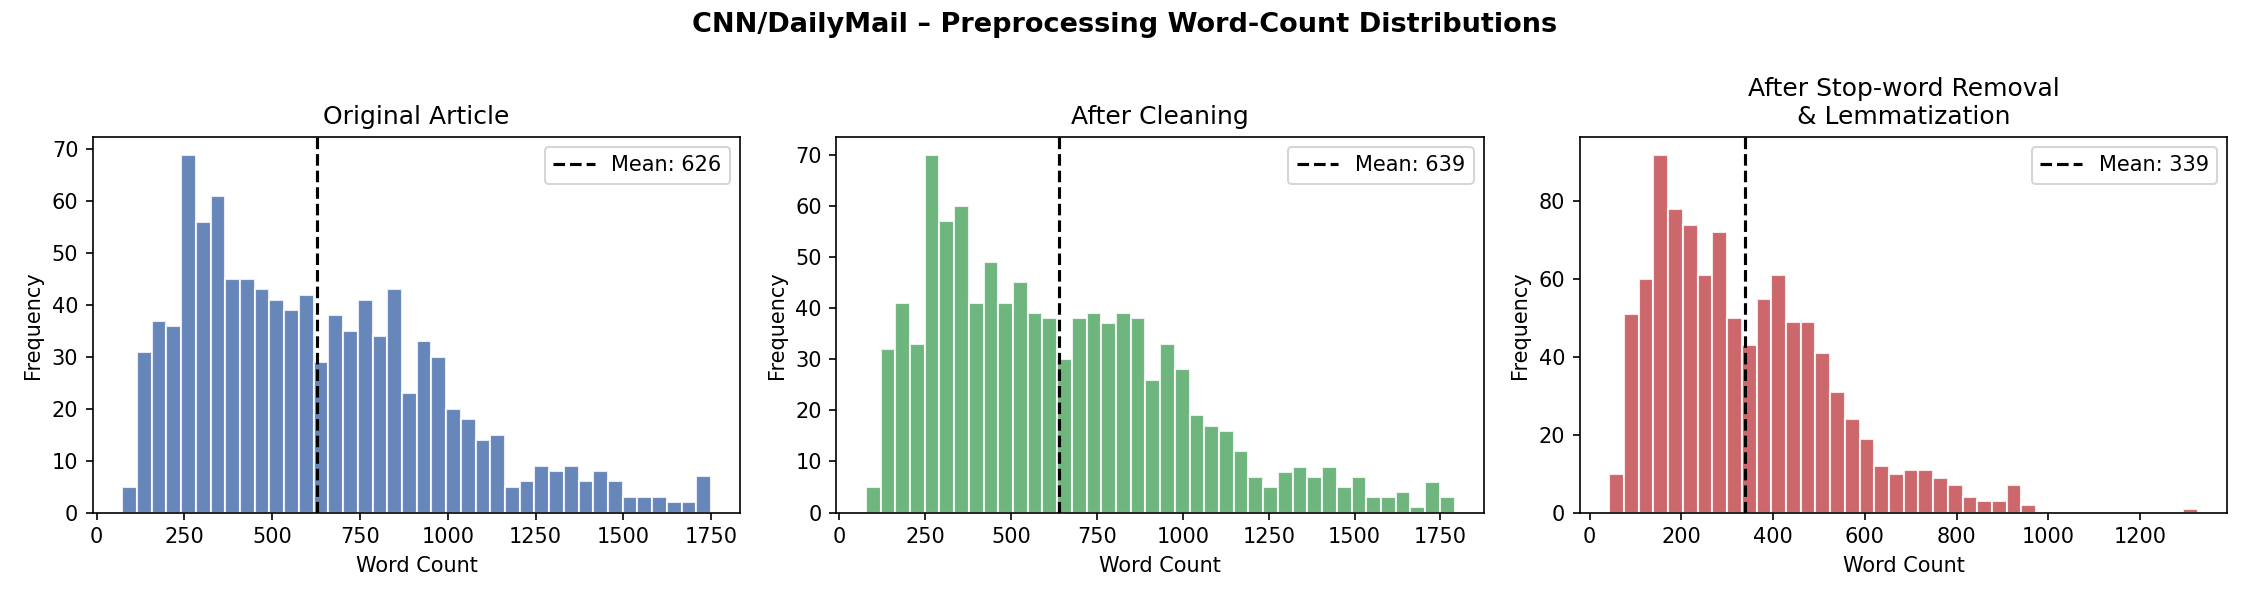
\includegraphics[width=\columnwidth]{outputs/preprocessing_wordcount.png}
    \caption{Word count distributions at three preprocessing stages:
             original article, after cleaning, and after stop-word
             removal and lemmatization.}
    \label{fig:preproc}
\end{figure}

% ─────────────────────────────────────────────────────────────────────
\section{Conclusion}
\label{sec:conclusion}

This paper presented a comprehensive comparison of six text summarization
models on the CNN/DailyMail benchmark. The key findings are:

\begin{enumerate}
    \item \textbf{BART-large-cnn is the best overall model}, achieving
          ROUGE-1 F1 of 34.55\%, ROUGE-2 F1 of 14.51\%, and ROUGE-L F1
          of 24.69\%. It wins against Lead-3 on 69\% of individual
          samples, confirming the value of fine-tuning on domain-specific
          data.

    \item \textbf{Lead-3 is a surprisingly strong baseline}, achieving
          ROUGE-1 F1 of 29.47\% --- higher than TextRank, LSA, and
          LexRank --- due to the inverted-pyramid structure of
          CNN/DailyMail articles.

    \item \textbf{Abstractive models outperform extractive models} by
          6.30\% on average ROUGE-1 F1 (32.97\% vs.\ 26.67\%),
          demonstrating the advantage of generative approaches.

    \item \textbf{T5-small (31.38\% R1-F1) beats Lead-3 (29.47\%)}
          despite being a general-purpose model not fine-tuned on
          CNN/DailyMail, showing the power of large-scale pre-training.

    \item \textbf{LSA is the weakest extractive model} (22.50\% R1-F1),
          as its topic-based scoring does not align well with the
          positional bias of this dataset.

    \item \textbf{LexRank marginally outperforms TextRank} (27.42\%
          vs.\ 27.28\% R1-F1) due to IDF-weighted similarity better
          capturing term importance.
\end{enumerate}

\noindent\textbf{Limitations.}
Abstractive models were evaluated on only 200 samples due to CPU
inference time ($\sim$27 minutes for BART on 200 samples). Additionally,
ROUGE measures lexical overlap and does not capture semantic correctness
or factual accuracy.

\noindent\textbf{Future Work.}
Future directions include: (1) evaluating PEGASUS \cite{zhang2020} and
PRIMERA for comparison; (2) fine-tuning T5-small on CNN/DailyMail to
close the gap with BART; (3) incorporating BERTScore for semantic
evaluation; (4) extending to multi-document summarization.

% ─────────────────────────────────────────────────────────────────────
\section*{GitHub Repository}

The full source code, scripts, and generated outputs for this project are
available at:\\
\url{https://github.com/<your-username>/NLP_CA_3_miniproject}

% ─────────────────────────────────────────────────────────────────────
\begin{thebibliography}{00}

\bibitem{luhn1958}
H.~P. Luhn, ``The automatic creation of literature abstracts,''
\textit{IBM Journal of Research and Development}, vol.~2, no.~2,
pp.~159--165, 1958.

\bibitem{edmundson1969}
H.~P. Edmundson, ``New methods in automatic extracting,''
\textit{Journal of the ACM}, vol.~16, no.~2, pp.~264--285, 1969.

\bibitem{mihalcea2004}
R.~Mihalcea and P.~Tarau, ``TextRank: Bringing order into texts,''
in \textit{Proc. EMNLP}, 2004, pp.~404--411.

\bibitem{erkan2004}
G.~Erkan and D.~R. Radev, ``LexRank: Graph-based lexical centrality as
salience in text summarization,''
\textit{Journal of Artificial Intelligence Research}, vol.~22,
pp.~457--479, 2004.

\bibitem{gong2001}
Y.~Gong and X.~Liu, ``Generic text summarization using relevance measure
and latent semantic analysis,''
in \textit{Proc. SIGIR}, 2001, pp.~19--25.

\bibitem{hermann2015}
K.~M. Hermann, T.~Kocisky, E.~Grefenstette, L.~Espeholt, W.~Kay,
M.~Suleyman, and P.~Blunsom, ``Teaching machines to read and comprehend,''
in \textit{Advances in Neural Information Processing Systems (NeurIPS)},
vol.~28, 2015.

\bibitem{nallapati2016}
R.~Nallapati, B.~Zhou, C.~dos Santos, C.~Gulcehre, and B.~Xiang,
``Abstractive text summarization using sequence-to-sequence RNNs and
beyond,''
in \textit{Proc. CoNLL}, 2016, pp.~280--290.

\bibitem{sutskever2014}
I.~Sutskever, O.~Vinyals, and Q.~V. Le, ``Sequence to sequence learning
with neural networks,''
in \textit{Advances in Neural Information Processing Systems (NeurIPS)},
vol.~27, 2014.

\bibitem{bahdanau2015}
D.~Bahdanau, K.~Cho, and Y.~Bengio, ``Neural machine translation by
jointly learning to align and translate,''
in \textit{Proc. ICLR}, 2015.

\bibitem{rush2015}
A.~M. Rush, S.~Chopra, and J.~Weston, ``A neural attention model for
abstractive sentence summarization,''
in \textit{Proc. EMNLP}, 2015, pp.~379--389.

\bibitem{see2017}
A.~See, P.~J. Liu, and C.~D. Manning, ``Get to the point: Summarization
with pointer-generator networks,''
in \textit{Proc. ACL}, 2017, pp.~1073--1083.

\bibitem{raffel2020}
C.~Raffel, N.~Shazeer, A.~Roberts, K.~Lee, S.~Narang, M.~Matena,
Y.~Zhou, W.~Li, and P.~J. Liu, ``Exploring the limits of transfer
learning with a unified text-to-text transformer,''
\textit{Journal of Machine Learning Research}, vol.~21, no.~140,
pp.~1--67, 2020.

\bibitem{lewis2020}
M.~Lewis, Y.~Liu, N.~Goyal, M.~Ghazvininejad, A.~Mohamed, O.~Levy,
V.~Stoyanov, and L.~Zettlemoyer, ``BART: Denoising sequence-to-sequence
pre-training for natural language generation, translation, and
comprehension,''
in \textit{Proc. ACL}, 2020, pp.~7871--7880.

\bibitem{lin2004}
C.~Y. Lin, ``ROUGE: A package for automatic evaluation of summaries,''
in \textit{Text Summarization Branches Out}, 2004, pp.~74--81.

\bibitem{zhang2020}
J.~Zhang, Y.~Zhao, M.~Saleh, and P.~J. Liu, ``PEGASUS: Pre-training with
extracted gap-sentences for abstractive summarization,''
in \textit{Proc. ICML}, 2020, pp.~11328--11339.

\end{thebibliography}

\end{document}
